
\chapter{Domain Background}




Kepler is a space observatory launched by NASA in 2009 to discover Eath-sized exoplanets orbiting other stars  \cite{2010ApJ...713L..87J}. Kepler mission developed several decades to answer the centuries-old question: How frequent are other Earth-like planets in Milkyway galaxy? In particular, what is the frequency of Earth-size planets in the Habitable-Zone of solar-like stars? There are three different types of exoplanets are common in our universe: gas giants, hot-super-Earths in short period orbits, and ice giants. The challenge is to find the terrestrial planets that are in the habitable zone of their stars where liquid water might exist on the surface of the planet.

The scientific objective of the Kepler mission is to explore the structure and diversity of planetary systems. This mission surveys a large sample of stars to determine the percentage of terrestrial and large planets that are in or near the habitable zone of a wide variety of stars and determine the distribution of size and shapes of the orbits of these planets. Kepler mission also estimates how many planets are in multiple-star systems. After collecting a large number of data points, using many techniques scientists determine the properties of those stars that harbor planarity systems including the planets itself. 

\section{Scentific Goals and Objectives of the Kepler Mission}

The primary goal of the Kepler Mission is to survey our region of the Milky Way galaxy to discover hundreds of Earth-size or larger planets in or near the habitable zone of solar-like stars and determine the existence of solar system like planetary systems \cite{2014PNAS..11112647B}. The scientific objective of the Kepler Mission is to explore the structure and diversity of extrasolar planetary systems. This is achieved by observing a large sample of stars to:
\begin{itemize}
  \item Determine the frequency of terrestrial and larger planets in or near the habitable zone of a wide variety of stellar spectral types of stars. 
  \item Determine the distribution of the size of planets and the size of the planet’s orbits.
  \item Estimate the frequency of planets in multiple star systems.
  \item Determine the distributions of orbital sizes, their light reflection properties (albedo), size, and density of
short-period giant planets.
  \item Identify additional members of each photometrically discovered planetary system using complementary techniques. 
  \item Determine the properties of those stars that harbor planetary systems. The spectral type, luminosity, and composition for each star showing transits are obtained from ground-based observations.
  \item Asteroseismology analysis of the data will be used to determine the mass, age, and size of the stars and astrometric analysis of the data will be used to calculate their distances, which also is used to calculate the size of the stars.
\end{itemize}

\section{Habitable Zone}

Habitable Zone is the range in the distance from a star where liquid water could exist on the surface of a planet orbiting a star that possibly supports life. Liquid water is essential to all life on Earth, and so the definition of a habitable zone is based on the hypothesis that extraterrestrial life would share this requirement \cite{2014ApJ...787L..29K}. This is a very traditional definition, as a planet surface temperature may depend on other factors such as greenhouse gas abundance, its reflectivity, atmospheric and oceanic circulation, radioactive decay, and tidal heating within the planet. These energy sources can be easily allowed the planet to have subsurface liquid water reservoirs.  Jupiter's moon Europa has liquid water ocean tens of kilometers below its surface that may well be habitable for some organisms. More than 20 planets, including the nearest extrasolar planet, Proxima Centauri b \cite{2016Natur.536..437A}, have been found that are both roughly Earth-sized and orbiting within a habitable zoned of their stars. 

\section{The Transit Method of Detecting Extrasolar Planets}

The Kepler mission detecs exoplanets using transit photometry \cite{2000ApJ...529L..45C}. When a planet passes in front of a star as a view from Earth, the event is call a ``{\emph {transit}}''. For example, we can observe an occasional Venus or Mercury transit from Earth as a small black dot creeping across the Sun. During this transit, the transiting planet block the starlight and dips the brightness of the star. When this happen, we say the planet transit the star, and can be detect using transit phometry. During transit, raw data is collected in the form of a sequence of stellar images, which are processed in to "light-curves" tracking the brightness of a star over time. Light-curves are graphs that show the brightness of an object over a period. 

\begin{figure}[!h]
\begin{center}
        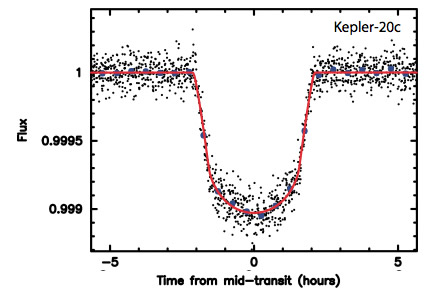
\includegraphics[width=0.6\textheight]{img/k20c.jpg}
        \caption{The light curve shown here was made from brightness data gathered by the Kepler Mission for discovery of planet Kepler-20c.
Image Credit: NASA}  \label{fig:lightcurve}
\end{center}
\end{figure}

Figure \ref{fig:lightcurve} shows the light curve made from the brightness data from Kepler Mission for the discovery of a planet named \emph{Kepler-20c}. Data clearly show the flux of the host star drop notability when the planet is in transit. This is the primary signature we are looking in the transit photometry to discover planets that are in orbits around stars. These planets create this photometric signature periodically while they are orbiting around the star. To make things more complicated, the light curves of some other objects also create similar photometric signatures: eclipsing binaries stars, certain other variable stars. During the classification stage, we need to classify these object as false positives. 


\section{Project  Proporsal and Motivation}
NASA's Kepler mission search for extrasolar planets has collected data from hundreds of thousands of star systems. Processing these large amounts of data, so far mission discovered 4,696 candidate exoplanets and 2,331 of them are confirmed as exoplanets leaving many more planet candidates to be confirmed in the dataset. These potential planetary candidates are searching using an algorithm that looks for periodic planetary transit in the light curves, but spurious intensity dips and other noise in the data due to non-planetery stellar variability has led to high false positive rates for detecting transits. As the initial planetary candidates found by this search method require extensive and costly subsequent validation, there is a need to reduce the error rate in exoplanet candidate identification. This exoplanet candidate data set refer to as Kepler Object of Interest (KOI). I present an algorithm (Multilayered Neural Network - MNN) to classify KOI as confirmed exoplanets or false positives using publically available data. MNN uses previously generated features extracted from the lightcurve time-series data, as well as newly generated autocorrelation features derived from the time-series specifically during the planet transits. 

NASA launched the Kepler mission when I was an undergraduate student (Physics major) in 2009. Since the day the mission has been initiated, I closely follow the mission updates.  I have moved to upstate NY to pursue my graduate studies in theoretical astrophysics (MS thesis in Numerical Relativity). Durig this time I have attended numerous scientific talks given by Kepler fellowship researchers at the University explaining and exploring the Kepler dataset. There are some groups are already using machine learning techniques to classify the Kepler data while others are developing more manual and careful procceses to extract planetary candidates. After taking the Udacity machine learning nano degree, it is natural for me to think of applying machine learning techniques to the Kepler dataset and see if that can improve the classification of planetary candidates. 
